\chapter{Introducción}
% Te escribo aquí el hilo conductor que tienes que seguir, con la filosofía siempre de "una idea, un párrafo":

\section{Contexto}

%1- La IA lleva muchos años en nuestras vidas: ejemplos medio antiguos.
La \ac{IA} ha tenido un impacto significativo en nuestro día a día, aunque a menudo de manera imperceptible. Desde la personalización de recomendaciones de productos en línea hasta encontrar el trayecto óptimo para moverte de un punto a otro en aplicaciones de mapas, la \ac{IA} lleva más de 20 años estando presente en varios aspectos de nuestra vida cotidiana.

%2- Pero últimamente está entrando de lleno y a nuestro día a día: chatGPT, etc. 
Sin embargo, ahora está más presente que nunca. Con la aparición de productos como chatGPT, asistentes de voz como Alexa o Siri, sistemas de reconocimiento facial como FaceID o la conducción autónoma como Tesla Autopilot, la \ac{IA} se ha convertido que una parte fundamental de la vida de muchas personas. También ha aumentado enormemente el interés general, tanto de personas particulares como de empresas, por esta tecnología con el fin de aplicarla a todas las áreas posibles maximizando el beneficio producido por su uso.


% 3- Esto puede ser muy bueno, pero muy ¡PELIGROSO! Hay ciertos contextos (educación, salud, democracia, cultura) donde hay que tener cuidado (high risk AI scenarios según EU Act). 
Aunque aún se está explorando el potencial de la \ac{IA} en varios campos, hay una creciente preocupación sobre cómo sistemas de \ac{IA} no supervisados por humanos pueden causar un impacto negativo en áreas más delicadas como la educación, salud, democracia, justicia, cultura o ciencia. Esto ha llevado a la definición de \textit{High-Risk AI Systems} por parte de \textit{EU AI Act}~\cite{euact}, los cuales son sistemas que pueden suponer un riesgo a los derechos fundamentales de las personas o a su integridad, como sistemas que procesen datos biométricos o aquellos usados en vehículos.

% 4- En este contexto surge Safe AI, trustworhy AI con los siguientes principios (coger el dibujo que usé en mi tesis, puedes citarlo tal cual la fuente).
En este contexto, emergen los conceptos de sistemas de \textit{Trustworthy AI} o \ac{IA} confiable y \textit{Responsible AI}~\cite{trusworth}. Los sistemas de \textit{Trustworthy AI} están basados en siete requisitos técnicos que se deben de mantener durante durante todo el ciclo de vida del sistema de \ac{IA}: 
\begin{enumerate}
    \item Supervisión e inspección humana.
    \item Robustez y seguridad.
    \item Privacidad y gobernanza de los datos.
    \item Transparencia.
    \item Diversidad, no discriminación y equidad.
    \item Bienestar social y ambiental.
    \item Rendición de cuentas.
\end{enumerate}

Estos requisitos están basados en tres pilares fundamentales: (1) legalidad, (2) ética, y (3) robustez, tanto desde perspectivas técnicas como sociales. Estos requisitos y sus pilares quedan ilustrados en la Figura~\ref{fig:tai}.
\begin{figure}
    \centering
    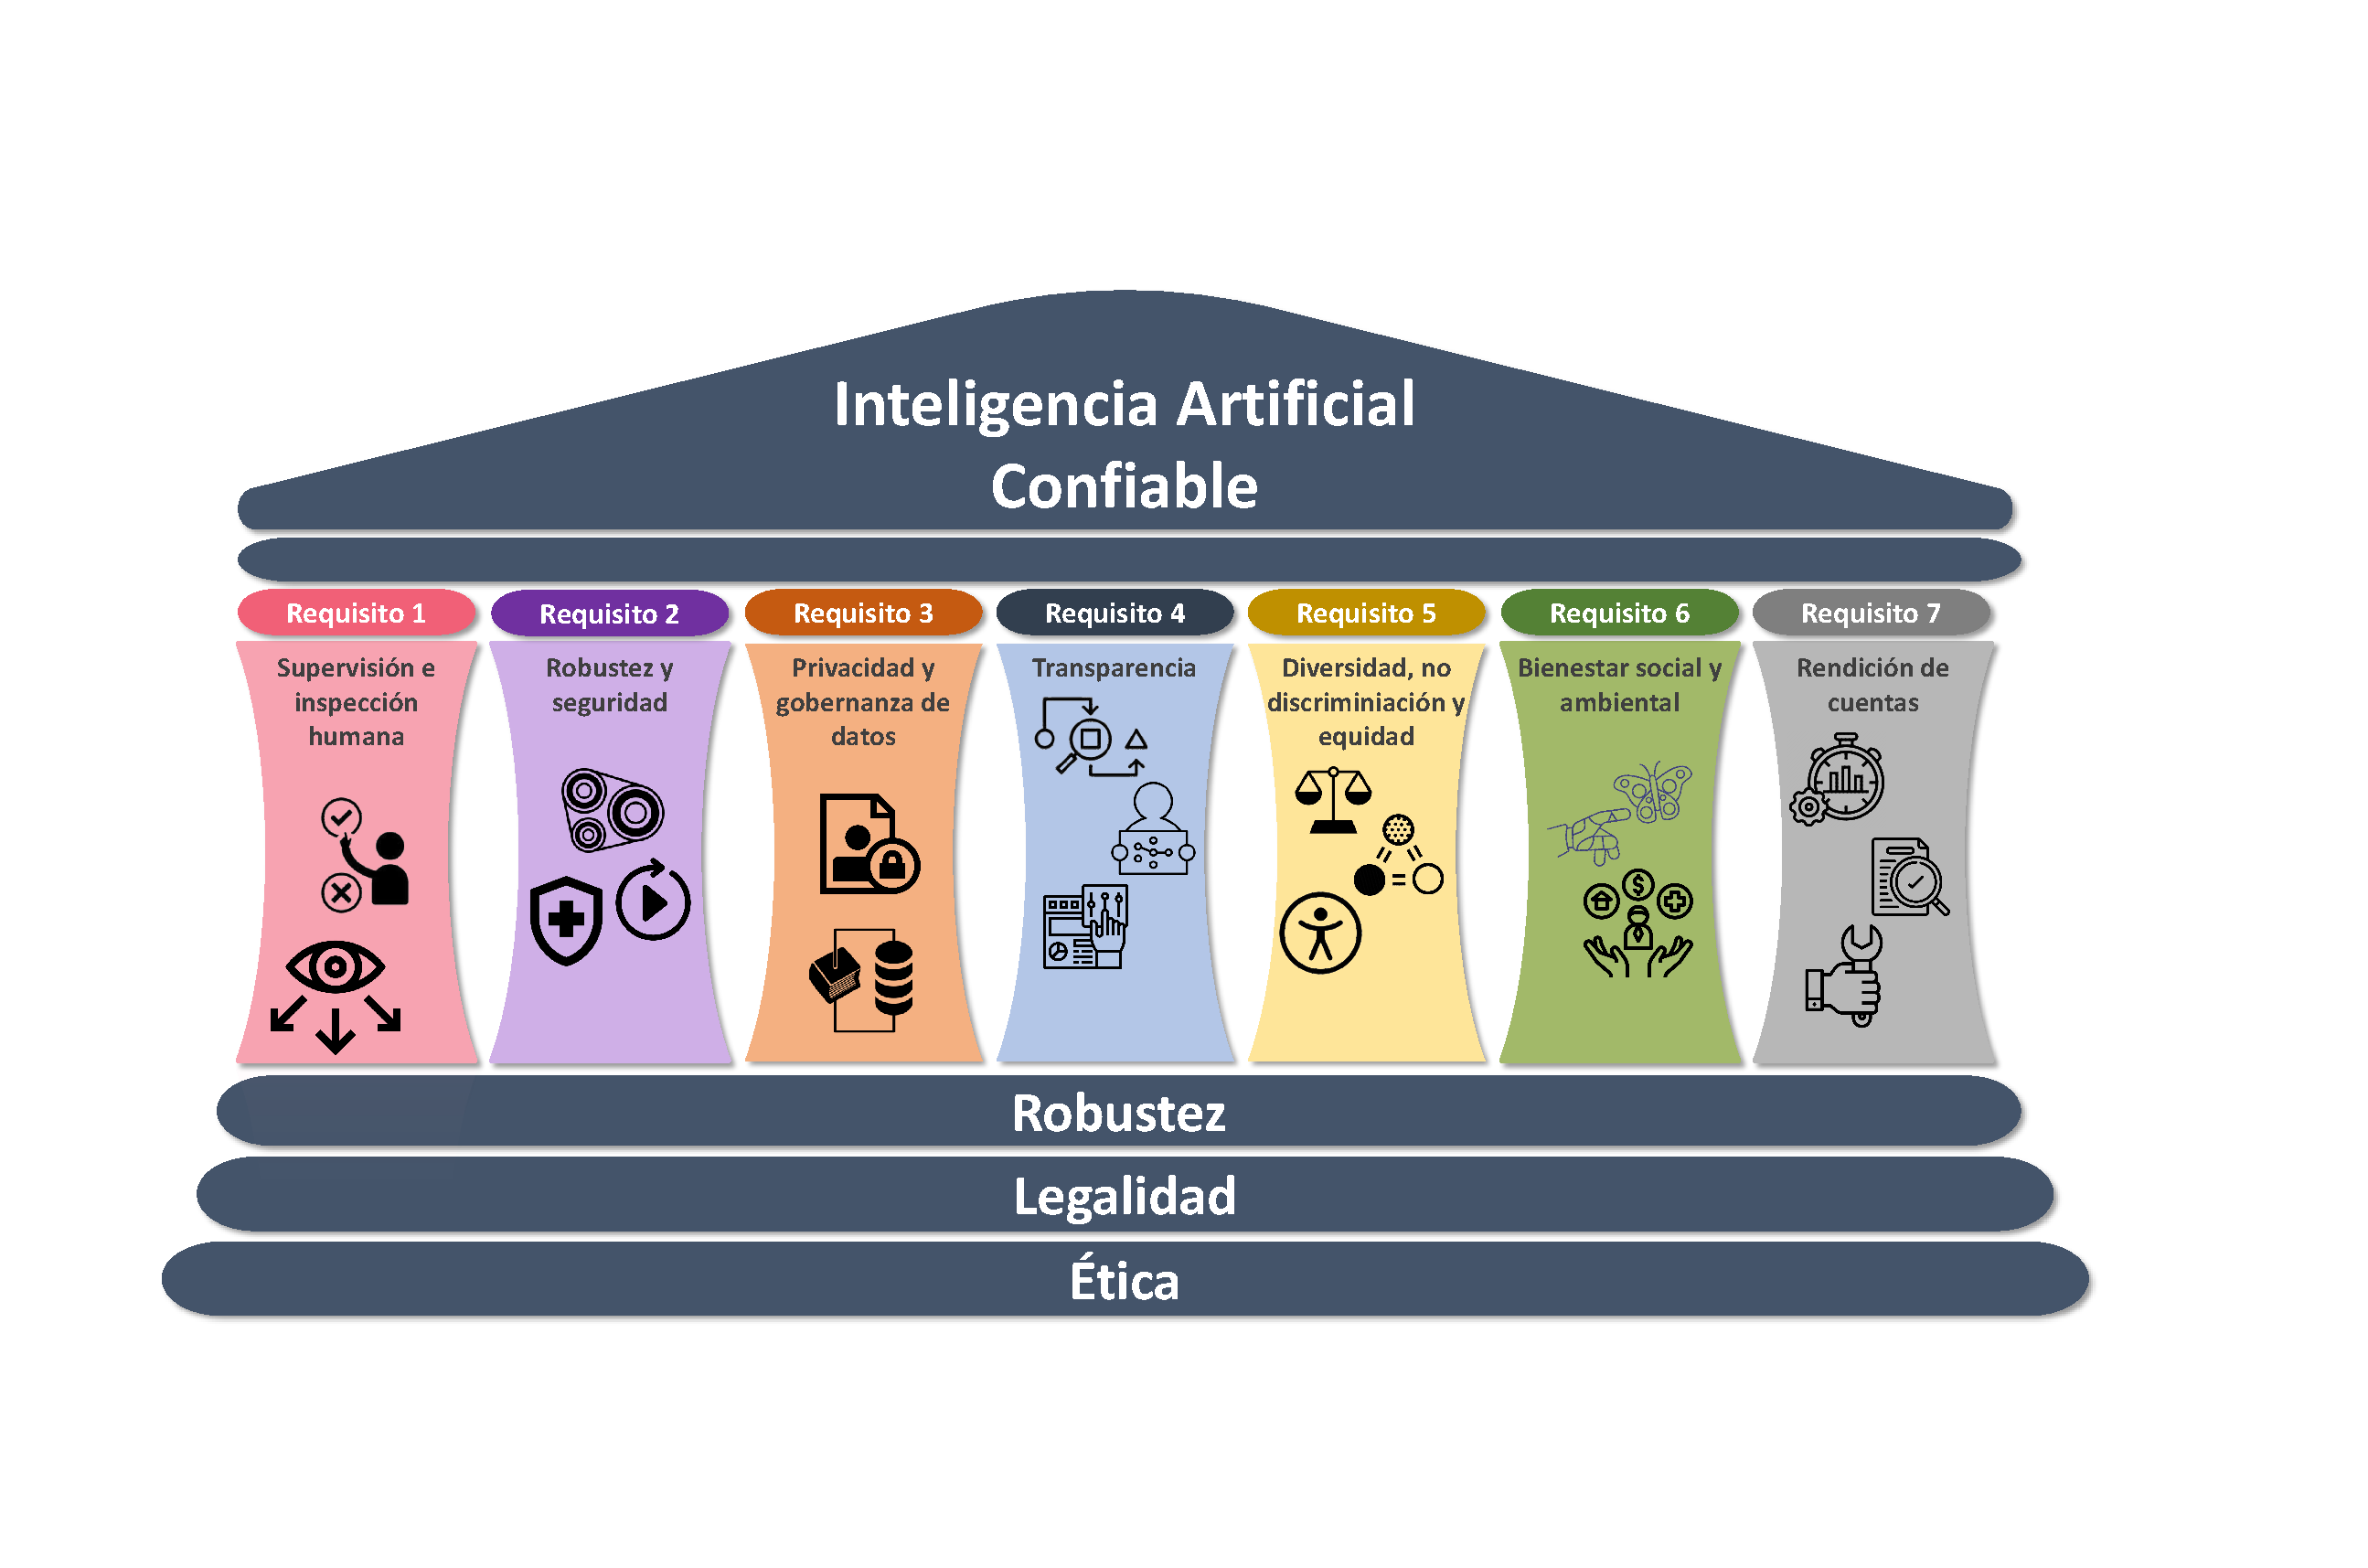
\includegraphics[width=\textwidth]{figuras/TAI.pdf}
    \caption{Diagrama de los requisitos técnicos de un sistema de \textit{Trusworthy AI}. Fuente:~\cite{diaz-tai}.}
    \label{fig:tai}
\end{figure}

% 5- Uno de los principales pialres para asegurar una IA segura y confiable: es la privacidad. En este contexto surge tanto el FL como la blockchain.
Uno de los requisitos técnicos de estos sistemas es garantizar la privacidad. Para ello, en 2016 e impulsado por Google, aparece el concepto de \ac{FL}~\cite{mcmahan-2023}, un paradigma de aprendizaje que permite el entrenamiento distribuido asegurando la privacidad de los datos. También durante este tiempo se aumenta el interés de las masas en las tecnologías \textit{blockchain}, tecnologías que permiten el registro digital descentralizado de transacciones compartidas entre una red que es inmutable, en parte impulsadas por el éxito de Bitcoin~\cite{bitcoin}.

\section{Motivación}

% 6- Parrafito super divulgativo de lo que es el FL y cómo ayuda.
Por su parte, el \ac{FL} permite el entrenamiento de un modelo distribuido sin que los clientes tengan que compartir sus datos privados con ninguna entidad. Para ello cada cliente entrena de manera local un modelo con sus datos personales, siendo este modelo el que luego es compartido con un servidor central, que finalmente agrega todos los resultados de los clientes para obtener un nuevo modelo global. \ac{FL} también incluye más ventajas como costes reducidos en comunicación o robustez respecto a otras alternativas distribuidas.

% 7- Parrafito super divulgativo de lo que es la blockchain y cómo ayuda.
Por otro lado, las tecnologías \textit{blockchain} ofrecen un esquema distribuido para computación~\cite{duc-2023} donde los datos son verificables e inmutables por todas las entidades mediante el uso de funciones criptográficas. A esto hay que añadir que es un sistema descentralizado donde no hay un servidor central, por lo que no hay un único servidor que sea vulnerable a ataques. Otros beneficios de estas tecnologías es una alta escalabilidad y facilidad para rastrear cambios a los datos compartidos~\cite{survey-blockchain}.

% 8- PERO, el FL es vulenrable a ataques adversarios ohhhhhhhhhhhh :(  Y aunque se ha intentado solucionar de muchísimas maneras, no se ha conseguido cubrir esta vulnerabilidad al 100\%.
Debido a estas características, el \ac{FL} se ha empleado en muchas situaciones con éxito~\cite{tutorial-nuria}. Sin embargo, al igual que cualquier modelo de \ac{AA}, es sensible a ataques. Se conocen varios tipos de ataques adversarios, enfocándose tanto en la funcionalidad del modelo como en la privacidad de los datos. Particularmente esto es una vulnerabilidad del \ac{FL}, debido a que al no tener acceso a los datos del entrenamiento, no se pueden aplicar técnicas de inspección de datos por lo que estos ataques se vuelven mucho más difíciles de mitigar. Son muchas las propuestas para mitigar estos ataques~\cite{survey-nuria-2023} pero todavía no se ha logrado solucionar al completo esta vulnerabilidad.

%9- Existen trabajos de FL + blockchain, y juntas pueden ayudarse para esto.
Es por ello que muchos trabajos han desarrollado maneras de combinar la tecnología \ac{FL} y \textit{blockchain}~\cite{kim-2020-blockfl, qu-2021-pofl, zhu-2023-blockfed} con aplicabilidad a \ac{IoT} industrial, detección de anomalías o resistencia a fallos de dispositivos. Uno de los principales argumentos para esto ha sido el de ofrecer una resistencia ante distintos tipos de ataques.

\section{Propuesta}

% 10- Hipótesis: PoFL. Pero tiene debilidades :(
En este trabajo exponemos la hipótesis de que \ac{PoFL}, un mecanismo de consenso diseñado para la combinación entre \ac{FL} y \textit{blockchain} con el fin de mejorar la eficiencia energética del sistema, podría ser un mecanismo viable de defensa contra ciertos ataques a un esquema federado. Sin embargo, esta hipótesis consta de algunos requisitos restrictivos sobre el escenario, no siendo aplicable de forma generalizada como mecanismo de defensa.

% 11- Propuesta: KFC.
Impulsados por estas limitaciones, proponemos la principal aportación de este trabajo, \ac{KFC}, una nueva arquitectura de \ac{FL} y \textit{blockchain} que tiene como objetivo el ofrecer una capa de seguridad robusta en los escenarios en los que \ac{PoFL} no se considera una defensa consistente.

% 12- Entorno experimentso que usamos muy resumido en un parrafito
Para verificar nuestras hipótesis, hemos entrenado tres modelos de clasificación de imágenes en distintos conjuntos de datos y en ambos escenarios: (1) cumpliendo las hipótesis necesitadas para \ac{PoFL} y (2) cuando estas restricciones no se cumplen, ambos bajo ataques hacia la funcionalidad del modelo, siendo estos un ataque de \textit{backdoor} y un ataque bizantino. También hacemos una comparación con arquitecturas clásicas en la literatura para verificar los resultados.

% 13- Resultados obtenidos: somos los putos fucking amos!!!!
Los resultados de los experimentos nos indican que, cumpliendo las hipótesis, \ac{PoFL} resulta ser eficaz y logra mitigar los ataques. Sin embargo, en caso de que no se cumplan, \ac{PoFL} se muestra completamente vulnerable ante estos ataques. Por el contrario, \ac{KFC} demuestra ser robusto, mitigando todos los ataques en todos los escenarios sin ninguna pérdida de rendimiento o compromiso con la seguridad del modelo, postulándose así como un método excelente para la defensa en esquemas federados.

\section{Estructura}

Esta memoria se organiza de la siguiente manera:
\begin{itemize}
    \item Primero hablaremos de todos los conceptos previos para hablar nuestra propuesta en la Parte~\ref{sec:preliminares}. Esta parte incluye:
    \begin{itemize}
        \item Una introducción al álgebra lineal en la Sección~\ref{sec:algebra}.
        \item Una introducción a la probabilidad y teoría de la información en la Sección~\ref{sec:inferencia}.
        \item Una introducción a la optimización no lineal sin restricciones en la Sección~\ref{sec:optim}.
        \item Un estudio del operador de agregación Krum en la Sección~\ref{sec:krum}.
        \item Una introducción a la teoría del aprendizaje en la Sección~\ref{sec:aa}.
        \item Una introducción al \textit{Deep Learning} en la Sección~\ref{sec:deep}.
    \end{itemize}
    \item Una vez dados los conceptos previos, podemos introducir conceptos más avanzados en la Parte~\ref{sec:fundamentosAaBl}.
    \begin{itemize}
        \item Hablaremos de \ac{FL} en la Sección~\ref{sec:fl}.
        \item Introduciremos el concepto de \textit{blockchain} en la Sección~\ref{sec:blockchain}.
    \end{itemize}
    \item Una vez explicados todos los conceptos necesarios, hablaremos de nuestra propuesta en la Parte~\ref{sec:kfc}.
    \begin{itemize}
        \item Empezaremos hablando sobre cómo combinar \textit{Blockchain} y \ac{FL} en la Sección~\ref{sec:blockfed}.
        \item Expondremos nuestra propuesta en la Sección~\ref{sec:propuesta}.
        \item Plantearemos los experimentos realizados en la Sección~\ref{sec:experimentos}.
        \item Analizaremos los resultados en la Sección~\ref{sec:resultados}
    \end{itemize}
    \item Finalmente, hablaremos de las conclusiones del trabajo en la Sección~\ref{sec:conclusiones}.
\end{itemize}

